\newpage
\section{Polecenie 7}

\subsection{ZMODYFIKOWANA TABELA WYCIECZKI}
Zmiana struktury bazy danych, w tabeli wycieczki dodajemy redundantne pole
liczba\_wolnych\_miejsc

\begin{verbatim}
CREATE TABLE WYCIECZKI
(
  ID_WYCIECZKI          INT GENERATED ALWAYS AS IDENTITY NOT NULL
  ,NAZWA                 VARCHAR2(100)
  ,KRAJ                  VARCHAR2(50)
  ,DATA                  DATE
  ,OPIS                  VARCHAR2(200)
  ,LICZBA_MIEJSC         INT
  ,LICZBA_WOLNYCH_MIEJSC INT
  ,CONSTRAINT WYCIECZKI_PK PRIMARY KEY
    (
      ID_WYCIECZKI
    )
  ENABLE
);
\end{verbatim}

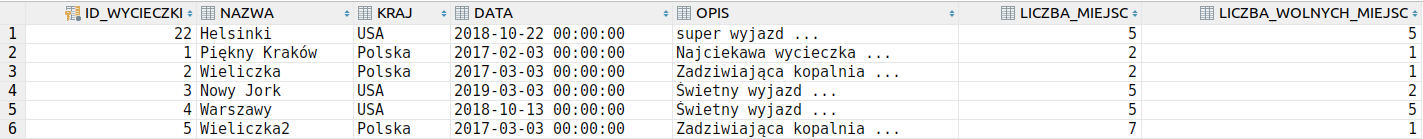
\includegraphics[width=\linewidth]{./images/zmodyfikowana_tabela_wycieczki.png}

\subsection{DOSTĘPNE WYCIECZKI 2}
Należy zmodyfikować zestaw widoków. Proponuję dodać kolejne widoki (np. z sufiksem 2), które
pobierają informację o wolnych miejscach z nowo dodanego pola.

\begin{verbatim}
CREATE VIEW DOSTEPNE_WYCIECZKI_2 AS
  SELECT *
  FROM WYCIECZKI W
  WHERE W.LICZBA_WOLNYCH_MIEJSC > 0
    AND W.DATA > (SELECT CURRENT_DATE FROM DUAL)
\end{verbatim}

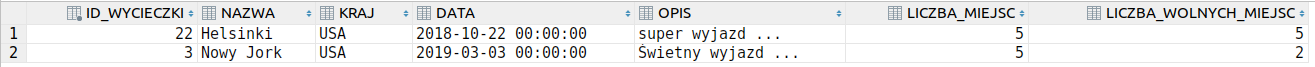
\includegraphics[width=\linewidth]{./images/dostepne_wycieczki_2.png}

\subsection{PRZELICZ}
Należy napisać procedurę przelicz która zaktualizuje wartość liczby wolnych miejsc dla już
istniejących danych

\begin{verbatim}
CREATE OR REPLACE PROCEDURE PRZELICZ AS
  BEGIN
    DECLARE
      VAL NUMBER;
    BEGIN
      FOR REC IN (SELECT W.ID_WYCIECZKI, W.LICZBA_MIEJSC -
                                         NVL((SELECT COUNT(*)
                                              FROM REZERWACJE R
                                              WHERE W.ID_WYCIECZKI = R.ID_WYCIECZKI
                                              GROUP BY R.ID_WYCIECZKI),
                                             0) LICZBA_MIEJSC_WOLNYCH
                  FROM WYCIECZKI W)
      LOOP
        UPDATE WYCIECZKI S
        SET S.LICZBA_WOLNYCH_MIEJSC = REC.LICZBA_MIEJSC_WOLNYCH
        WHERE S.ID_WYCIECZKI = REC.ID_WYCIECZKI;
      END LOOP;
    END;
  END;
\end{verbatim}

Sprawdzenie procedury przelicz następuje dalej.

\subsection{DOSTEPNE MIEJSCA 2}
Należy zmodyfikować warstwę procedur pobierających dane, podobnie jak w przypadku
widoków.

\begin{verbatim}
CREATE OR REPLACE FUNCTION DOSTEPNE_MIEJSCA_2(ID_W NUMBER)
  RETURN NUMBER
IS
  LICZBA_WOLNYCH_MIEJSC_ NUMBER;
  BEGIN
    SELECT W.LICZBA_WOLNYCH_MIEJSC INTO LICZBA_WOLNYCH_MIEJSC_ FROM WYCIECZKI W WHERE W.ID_WYCIECZKI = ID_W;
    RETURN LICZBA_WOLNYCH_MIEJSC_;
  END;
\end{verbatim}

\begin{minipage}{0.40\textwidth}
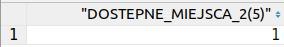
\includegraphics[width=\linewidth]{./images/dostepne_miejsca_2.png}
\end{minipage}

\subsection{DOSTEPNE WYCIECZKI 2}
\begin{verbatim}
CREATE OR REPLACE FUNCTION DOSTEPNE_WYCIECZKI_2_(KRAJ_ VARCHAR2, DATA_OD DATE, DATA_DO DATE)
  RETURN TAB_DOSTEPNE_WYCIECZKI PIPELINED
AS
  BEGIN
    FOR X IN (SELECT W.KRAJ, W.DATA
              FROM WYCIECZKI W
              WHERE W.LICZBA_WOLNYCH_MIEJSC > 0
                AND (SELECT CURRENT_DATE FROM DUAL) < W.DATA
                AND W.DATA BETWEEN DATA_OD AND DATA_DO
                AND W.KRAJ = KRAJ_)
    LOOP
      PIPE ROW (TYPE_DOSTEPNE_WYCIECZKI(X.KRAJ, X.DATA));
    END LOOP;
    RETURN;
  END;
\end{verbatim}

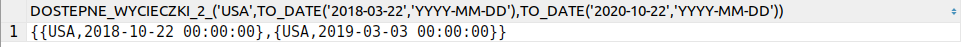
\includegraphics[width=\linewidth]{./images/dostepne_wycieczki_2_.png}

\subsection{DODAJ REZERWACJE 2}
Należy zmodyfikować procedury wprowadzające dane tak aby korzystały/aktualizowały pole
liczba\_wolnych\_miejsc w tabeli wycieczki
Najlepiej to zrobić tworząc nowe wersje (np. z sufiksem 

\begin{verbatim}
CREATE OR REPLACE PROCEDURE DODAJ_REZERWACJE_2(ID_W NUMBER, ID_O NUMBER)
AS
  BEGIN
    DECLARE
      WYCIECZKI NUMBER;
      OSOBA     NUMBER;
    BEGIN

      SELECT COUNT(W.ID_WYCIECZKI) INTO WYCIECZKI FROM WYCIECZKI W WHERE W.ID_WYCIECZKI = ID_W;
      SELECT O.ID_OSOBY INTO OSOBA FROM OSOBY O WHERE O.ID_OSOBY = ID_O;

      IF WYCIECZKI > 0 AND OSOBA > 0
      THEN
        INSERT INTO REZERWACJE (ID_WYCIECZKI, ID_OSOBY, STATUS) VALUES (ID_W, ID_O, 'N');
        BEGIN
          PRZELICZ();
        END;
      END IF;
    END;
  END;
\end{verbatim}

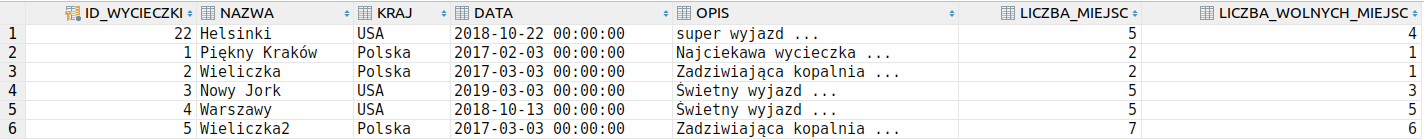
\includegraphics[width=\linewidth]{./images/dodaj_rezerwacje_2.png}

\begin{verbatim}
begin
  DODAJ_REZERWACJE_2(5, 2);
end;
\end{verbatim}
Po wykonaniu procedury:\\
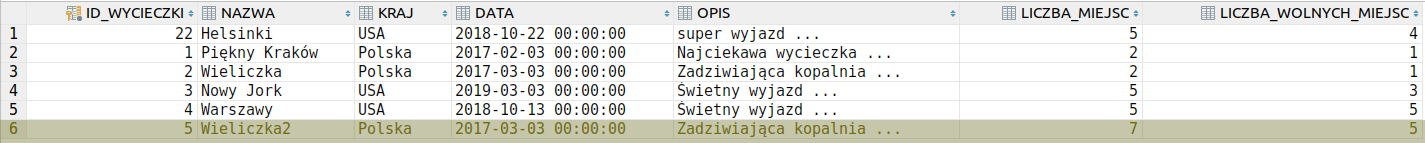
\includegraphics[width=\linewidth]{./images/dodaj_rezerwacje_2_.png}
Uaktualnione zostało pole LICZBA\_WOLNYCH\_MIEJSC, co powtwierdza poprawność działania procedury przelicz.
Tutaj wynik z tabeli REZERWACJE:\\ 
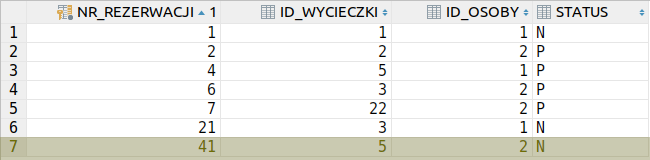
\includegraphics[width=\linewidth]{./images/dodaj_rezerwacje_2__.png}

\subsection{ZMIEN LICZBE MIEJSC 2}
\begin{verbatim}
CREATE PROCEDURE ZMIEN_LICZBE_MIEJSC_2(ID_WYCIECZKI_ NUMBER, NOWA_LICZBA_MIEJSC NUMBER)
AS
  BEGIN
    DECLARE
      CALKOWITA_LICZBA_MIEJSC NUMBER;
      DOSTEPNE_MIEJSCA_       NUMBER;
    BEGIN
      SELECT W.LICZBA_MIEJSC INTO CALKOWITA_LICZBA_MIEJSC FROM WYCIECZKI W WHERE W.ID_WYCIECZKI = ID_WYCIECZKI_;
      SELECT DOSTEPNE_MIEJSCA(ID_WYCIECZKI_) INTO DOSTEPNE_MIEJSCA_ FROM DUAL;
      IF (NOWA_LICZBA_MIEJSC >= (CALKOWITA_LICZBA_MIEJSC - DOSTEPNE_MIEJSCA_))
      THEN
        UPDATE WYCIECZKI W SET W.LICZBA_MIEJSC = NOWA_LICZBA_MIEJSC WHERE W.ID_WYCIECZKI = ID_WYCIECZKI_;
        BEGIN
          PRZELICZ();
        END;
      END IF;
    END;
  END;
\end{verbatim}

Po wykonaniu procedury:
\begin{verbatim}
begin
  ZMIEN_LICZBE_MIEJSC_2(5, 5);
end;
\end{verbatim}
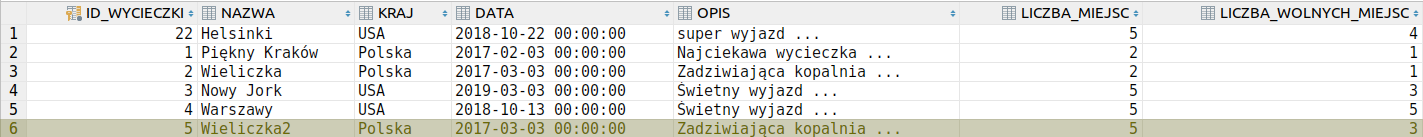
\includegraphics[width=\linewidth]{./images/zmien_liczbe_miejsc_2.png}



  